% Created by tikzDevice version 0.12.3.1 on 2022-09-24 18:17:45
% !TEX encoding = UTF-8 Unicode
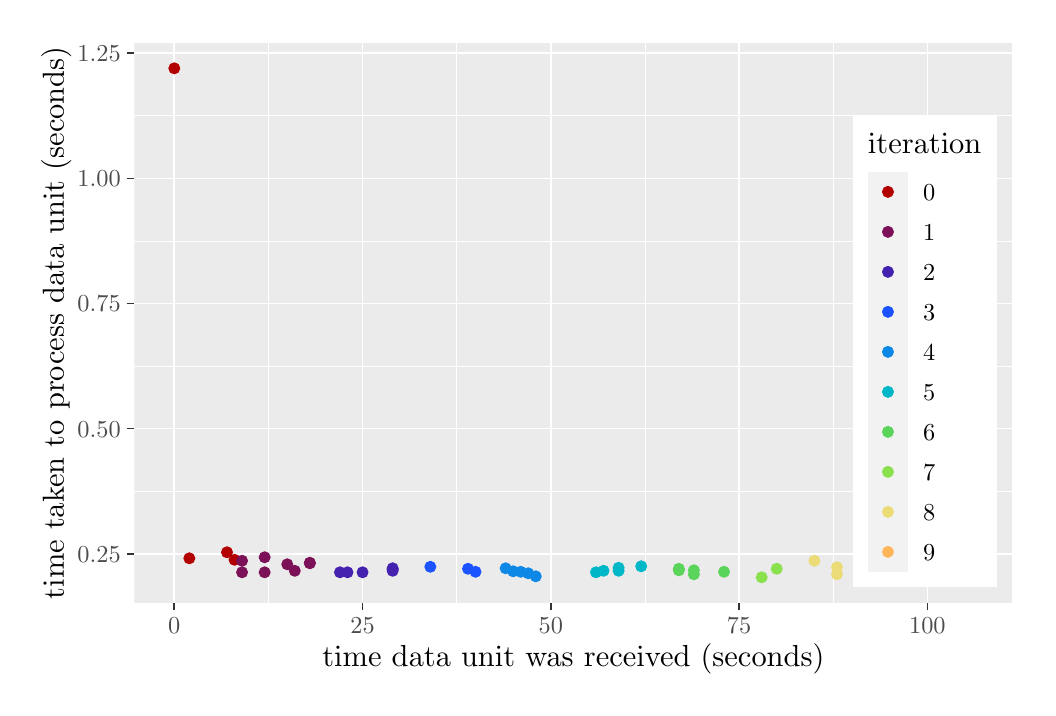
\begin{tikzpicture}[x=1pt,y=1pt]
\definecolor{fillColor}{RGB}{255,255,255}
\path[use as bounding box,fill=fillColor,fill opacity=0.00] (0,0) rectangle (361.35,238.49);
\begin{scope}
\path[clip] (  0.00,  0.00) rectangle (361.35,238.49);
\definecolor{drawColor}{RGB}{255,255,255}
\definecolor{fillColor}{RGB}{255,255,255}

\path[draw=drawColor,line width= 0.6pt,line join=round,line cap=round,fill=fillColor] (  0.00,  0.00) rectangle (361.35,238.49);
\end{scope}
\begin{scope}
\path[clip] ( 38.56, 30.69) rectangle (355.85,232.99);
\definecolor{fillColor}{gray}{0.92}

\path[fill=fillColor] ( 38.56, 30.69) rectangle (355.85,232.99);
\definecolor{drawColor}{RGB}{255,255,255}

\path[draw=drawColor,line width= 0.3pt,line join=round] ( 38.56, 70.99) --
	(355.85, 70.99);

\path[draw=drawColor,line width= 0.3pt,line join=round] ( 38.56,116.20) --
	(355.85,116.20);

\path[draw=drawColor,line width= 0.3pt,line join=round] ( 38.56,161.41) --
	(355.85,161.41);

\path[draw=drawColor,line width= 0.3pt,line join=round] ( 38.56,206.62) --
	(355.85,206.62);

\path[draw=drawColor,line width= 0.3pt,line join=round] ( 86.99, 30.69) --
	( 86.99,232.99);

\path[draw=drawColor,line width= 0.3pt,line join=round] (155.02, 30.69) --
	(155.02,232.99);

\path[draw=drawColor,line width= 0.3pt,line join=round] (223.05, 30.69) --
	(223.05,232.99);

\path[draw=drawColor,line width= 0.3pt,line join=round] (291.08, 30.69) --
	(291.08,232.99);

\path[draw=drawColor,line width= 0.6pt,line join=round] ( 38.56, 48.38) --
	(355.85, 48.38);

\path[draw=drawColor,line width= 0.6pt,line join=round] ( 38.56, 93.59) --
	(355.85, 93.59);

\path[draw=drawColor,line width= 0.6pt,line join=round] ( 38.56,138.80) --
	(355.85,138.80);

\path[draw=drawColor,line width= 0.6pt,line join=round] ( 38.56,184.01) --
	(355.85,184.01);

\path[draw=drawColor,line width= 0.6pt,line join=round] ( 38.56,229.22) --
	(355.85,229.22);

\path[draw=drawColor,line width= 0.6pt,line join=round] ( 52.98, 30.69) --
	( 52.98,232.99);

\path[draw=drawColor,line width= 0.6pt,line join=round] (121.01, 30.69) --
	(121.01,232.99);

\path[draw=drawColor,line width= 0.6pt,line join=round] (189.04, 30.69) --
	(189.04,232.99);

\path[draw=drawColor,line width= 0.6pt,line join=round] (257.07, 30.69) --
	(257.07,232.99);

\path[draw=drawColor,line width= 0.6pt,line join=round] (325.10, 30.69) --
	(325.10,232.99);
\definecolor{drawColor}{RGB}{179,0,0}
\definecolor{fillColor}{RGB}{179,0,0}

\path[draw=drawColor,line width= 0.4pt,line join=round,line cap=round,fill=fillColor] ( 52.98,223.80) circle (  1.96);

\path[draw=drawColor,line width= 0.4pt,line join=round,line cap=round,fill=fillColor] ( 58.42, 46.75) circle (  1.96);

\path[draw=drawColor,line width= 0.4pt,line join=round,line cap=round,fill=fillColor] ( 72.03, 48.92) circle (  1.96);

\path[draw=drawColor,line width= 0.4pt,line join=round,line cap=round,fill=fillColor] ( 74.75, 46.21) circle (  1.96);
\definecolor{drawColor}{RGB}{124,17,88}
\definecolor{fillColor}{RGB}{124,17,88}

\path[draw=drawColor,line width= 0.4pt,line join=round,line cap=round,fill=fillColor] ( 77.47, 41.69) circle (  1.96);

\path[draw=drawColor,line width= 0.4pt,line join=round,line cap=round,fill=fillColor] ( 77.47, 45.85) circle (  1.96);

\path[draw=drawColor,line width= 0.4pt,line join=round,line cap=round,fill=fillColor] ( 85.63, 47.12) circle (  1.96);

\path[draw=drawColor,line width= 0.4pt,line join=round,line cap=round,fill=fillColor] ( 85.63, 41.69) circle (  1.96);

\path[draw=drawColor,line width= 0.4pt,line join=round,line cap=round,fill=fillColor] ( 93.80, 44.58) circle (  1.96);

\path[draw=drawColor,line width= 0.4pt,line join=round,line cap=round,fill=fillColor] ( 96.52, 42.23) circle (  1.96);

\path[draw=drawColor,line width= 0.4pt,line join=round,line cap=round,fill=fillColor] (101.96, 44.95) circle (  1.96);

\path[draw=drawColor,line width= 0.4pt,line join=round,line cap=round,fill=fillColor] (101.96, 45.13) circle (  1.96);
\definecolor{drawColor}{RGB}{68,33,175}
\definecolor{fillColor}{RGB}{68,33,175}

\path[draw=drawColor,line width= 0.4pt,line join=round,line cap=round,fill=fillColor] (112.84, 41.69) circle (  1.96);

\path[draw=drawColor,line width= 0.4pt,line join=round,line cap=round,fill=fillColor] (115.57, 41.69) circle (  1.96);

\path[draw=drawColor,line width= 0.4pt,line join=round,line cap=round,fill=fillColor] (121.01, 41.69) circle (  1.96);

\path[draw=drawColor,line width= 0.4pt,line join=round,line cap=round,fill=fillColor] (131.89, 42.77) circle (  1.96);

\path[draw=drawColor,line width= 0.4pt,line join=round,line cap=round,fill=fillColor] (131.89, 43.14) circle (  1.96);

\path[draw=drawColor,line width= 0.4pt,line join=round,line cap=round,fill=fillColor] (131.89, 42.23) circle (  1.96);
\definecolor{drawColor}{RGB}{26,83,255}
\definecolor{fillColor}{RGB}{26,83,255}

\path[draw=drawColor,line width= 0.4pt,line join=round,line cap=round,fill=fillColor] (145.50, 43.68) circle (  1.96);

\path[draw=drawColor,line width= 0.4pt,line join=round,line cap=round,fill=fillColor] (159.11, 42.96) circle (  1.96);

\path[draw=drawColor,line width= 0.4pt,line join=round,line cap=round,fill=fillColor] (161.83, 41.87) circle (  1.96);
\definecolor{drawColor}{RGB}{13,136,230}
\definecolor{fillColor}{RGB}{13,136,230}

\path[draw=drawColor,line width= 0.4pt,line join=round,line cap=round,fill=fillColor] (172.71, 43.14) circle (  1.96);

\path[draw=drawColor,line width= 0.4pt,line join=round,line cap=round,fill=fillColor] (175.43, 42.05) circle (  1.96);

\path[draw=drawColor,line width= 0.4pt,line join=round,line cap=round,fill=fillColor] (178.15, 41.87) circle (  1.96);

\path[draw=drawColor,line width= 0.4pt,line join=round,line cap=round,fill=fillColor] (180.88, 41.33) circle (  1.96);

\path[draw=drawColor,line width= 0.4pt,line join=round,line cap=round,fill=fillColor] (183.60, 40.24) circle (  1.96);
\definecolor{drawColor}{RGB}{0,183,199}
\definecolor{fillColor}{RGB}{0,183,199}

\path[draw=drawColor,line width= 0.4pt,line join=round,line cap=round,fill=fillColor] (205.37, 41.69) circle (  1.96);

\path[draw=drawColor,line width= 0.4pt,line join=round,line cap=round,fill=fillColor] (208.09, 42.23) circle (  1.96);

\path[draw=drawColor,line width= 0.4pt,line join=round,line cap=round,fill=fillColor] (213.53, 42.23) circle (  1.96);

\path[draw=drawColor,line width= 0.4pt,line join=round,line cap=round,fill=fillColor] (213.53, 43.32) circle (  1.96);

\path[draw=drawColor,line width= 0.4pt,line join=round,line cap=round,fill=fillColor] (221.69, 43.86) circle (  1.96);
\definecolor{drawColor}{RGB}{90,212,90}
\definecolor{fillColor}{RGB}{90,212,90}

\path[draw=drawColor,line width= 0.4pt,line join=round,line cap=round,fill=fillColor] (235.30, 42.41) circle (  1.96);

\path[draw=drawColor,line width= 0.4pt,line join=round,line cap=round,fill=fillColor] (235.30, 42.96) circle (  1.96);

\path[draw=drawColor,line width= 0.4pt,line join=round,line cap=round,fill=fillColor] (240.74, 42.41) circle (  1.96);

\path[draw=drawColor,line width= 0.4pt,line join=round,line cap=round,fill=fillColor] (240.74, 40.97) circle (  1.96);

\path[draw=drawColor,line width= 0.4pt,line join=round,line cap=round,fill=fillColor] (251.63, 41.87) circle (  1.96);
\definecolor{drawColor}{RGB}{139,224,78}
\definecolor{fillColor}{RGB}{139,224,78}

\path[draw=drawColor,line width= 0.4pt,line join=round,line cap=round,fill=fillColor] (265.23, 39.88) circle (  1.96);

\path[draw=drawColor,line width= 0.4pt,line join=round,line cap=round,fill=fillColor] (270.68, 42.96) circle (  1.96);
\definecolor{drawColor}{RGB}{235,220,120}
\definecolor{fillColor}{RGB}{235,220,120}

\path[draw=drawColor,line width= 0.4pt,line join=round,line cap=round,fill=fillColor] (284.28, 45.85) circle (  1.96);

\path[draw=drawColor,line width= 0.4pt,line join=round,line cap=round,fill=fillColor] (292.45, 43.50) circle (  1.96);

\path[draw=drawColor,line width= 0.4pt,line join=round,line cap=round,fill=fillColor] (292.45, 40.97) circle (  1.96);

\path[draw=drawColor,line width= 0.4pt,line join=round,line cap=round,fill=fillColor] (308.77, 43.86) circle (  1.96);

\path[draw=drawColor,line width= 0.4pt,line join=round,line cap=round,fill=fillColor] (311.49, 42.77) circle (  1.96);
\definecolor{drawColor}{RGB}{255,181,90}
\definecolor{fillColor}{RGB}{255,181,90}

\path[draw=drawColor,line width= 0.4pt,line join=round,line cap=round,fill=fillColor] (314.22, 44.76) circle (  1.96);

\path[draw=drawColor,line width= 0.4pt,line join=round,line cap=round,fill=fillColor] (325.10, 44.58) circle (  1.96);

\path[draw=drawColor,line width= 0.4pt,line join=round,line cap=round,fill=fillColor] (335.99, 42.59) circle (  1.96);

\path[draw=drawColor,line width= 0.4pt,line join=round,line cap=round,fill=fillColor] (341.43, 42.96) circle (  1.96);
\end{scope}
\begin{scope}
\path[clip] (  0.00,  0.00) rectangle (361.35,238.49);
\definecolor{drawColor}{gray}{0.30}

\node[text=drawColor,anchor=base east,inner sep=0pt, outer sep=0pt, scale=  0.88] at ( 33.61, 45.35) {0.25};

\node[text=drawColor,anchor=base east,inner sep=0pt, outer sep=0pt, scale=  0.88] at ( 33.61, 90.56) {0.50};

\node[text=drawColor,anchor=base east,inner sep=0pt, outer sep=0pt, scale=  0.88] at ( 33.61,135.77) {0.75};

\node[text=drawColor,anchor=base east,inner sep=0pt, outer sep=0pt, scale=  0.88] at ( 33.61,180.98) {1.00};

\node[text=drawColor,anchor=base east,inner sep=0pt, outer sep=0pt, scale=  0.88] at ( 33.61,226.19) {1.25};
\end{scope}
\begin{scope}
\path[clip] (  0.00,  0.00) rectangle (361.35,238.49);
\definecolor{drawColor}{gray}{0.20}

\path[draw=drawColor,line width= 0.6pt,line join=round] ( 35.81, 48.38) --
	( 38.56, 48.38);

\path[draw=drawColor,line width= 0.6pt,line join=round] ( 35.81, 93.59) --
	( 38.56, 93.59);

\path[draw=drawColor,line width= 0.6pt,line join=round] ( 35.81,138.80) --
	( 38.56,138.80);

\path[draw=drawColor,line width= 0.6pt,line join=round] ( 35.81,184.01) --
	( 38.56,184.01);

\path[draw=drawColor,line width= 0.6pt,line join=round] ( 35.81,229.22) --
	( 38.56,229.22);
\end{scope}
\begin{scope}
\path[clip] (  0.00,  0.00) rectangle (361.35,238.49);
\definecolor{drawColor}{gray}{0.20}

\path[draw=drawColor,line width= 0.6pt,line join=round] ( 52.98, 27.94) --
	( 52.98, 30.69);

\path[draw=drawColor,line width= 0.6pt,line join=round] (121.01, 27.94) --
	(121.01, 30.69);

\path[draw=drawColor,line width= 0.6pt,line join=round] (189.04, 27.94) --
	(189.04, 30.69);

\path[draw=drawColor,line width= 0.6pt,line join=round] (257.07, 27.94) --
	(257.07, 30.69);

\path[draw=drawColor,line width= 0.6pt,line join=round] (325.10, 27.94) --
	(325.10, 30.69);
\end{scope}
\begin{scope}
\path[clip] (  0.00,  0.00) rectangle (361.35,238.49);
\definecolor{drawColor}{gray}{0.30}

\node[text=drawColor,anchor=base,inner sep=0pt, outer sep=0pt, scale=  0.88] at ( 52.98, 19.68) {0};

\node[text=drawColor,anchor=base,inner sep=0pt, outer sep=0pt, scale=  0.88] at (121.01, 19.68) {25};

\node[text=drawColor,anchor=base,inner sep=0pt, outer sep=0pt, scale=  0.88] at (189.04, 19.68) {50};

\node[text=drawColor,anchor=base,inner sep=0pt, outer sep=0pt, scale=  0.88] at (257.07, 19.68) {75};

\node[text=drawColor,anchor=base,inner sep=0pt, outer sep=0pt, scale=  0.88] at (325.10, 19.68) {100};
\end{scope}
\begin{scope}
\path[clip] (  0.00,  0.00) rectangle (361.35,238.49);
\definecolor{drawColor}{RGB}{0,0,0}

\node[text=drawColor,anchor=base,inner sep=0pt, outer sep=0pt, scale=  1.10] at (197.20,  7.64) {time data unit was received (seconds)};
\end{scope}
\begin{scope}
\path[clip] (  0.00,  0.00) rectangle (361.35,238.49);
\definecolor{drawColor}{RGB}{0,0,0}

\node[text=drawColor,rotate= 90.00,anchor=base,inner sep=0pt, outer sep=0pt, scale=  1.10] at ( 13.08,131.84) {time taken to process data unit (seconds)};
\end{scope}
\begin{scope}
\path[clip] (  0.00,  0.00) rectangle (361.35,238.49);
\definecolor{fillColor}{RGB}{255,255,255}

\path[fill=fillColor] (298.14, 36.35) rectangle (350.10,207.10);
\end{scope}
\begin{scope}
\path[clip] (  0.00,  0.00) rectangle (361.35,238.49);
\definecolor{drawColor}{RGB}{0,0,0}

\node[text=drawColor,anchor=base west,inner sep=0pt, outer sep=0pt, scale=  1.10] at (303.64,192.96) {iteration};
\end{scope}
\begin{scope}
\path[clip] (  0.00,  0.00) rectangle (361.35,238.49);
\definecolor{fillColor}{gray}{0.95}

\path[fill=fillColor] (303.64,171.93) rectangle (318.09,186.39);
\end{scope}
\begin{scope}
\path[clip] (  0.00,  0.00) rectangle (361.35,238.49);
\definecolor{drawColor}{RGB}{179,0,0}
\definecolor{fillColor}{RGB}{179,0,0}

\path[draw=drawColor,line width= 0.4pt,line join=round,line cap=round,fill=fillColor] (310.86,179.16) circle (  1.96);
\end{scope}
\begin{scope}
\path[clip] (  0.00,  0.00) rectangle (361.35,238.49);
\definecolor{fillColor}{gray}{0.95}

\path[fill=fillColor] (303.64,157.48) rectangle (318.09,171.93);
\end{scope}
\begin{scope}
\path[clip] (  0.00,  0.00) rectangle (361.35,238.49);
\definecolor{drawColor}{RGB}{124,17,88}
\definecolor{fillColor}{RGB}{124,17,88}

\path[draw=drawColor,line width= 0.4pt,line join=round,line cap=round,fill=fillColor] (310.86,164.70) circle (  1.96);
\end{scope}
\begin{scope}
\path[clip] (  0.00,  0.00) rectangle (361.35,238.49);
\definecolor{fillColor}{gray}{0.95}

\path[fill=fillColor] (303.64,143.02) rectangle (318.09,157.48);
\end{scope}
\begin{scope}
\path[clip] (  0.00,  0.00) rectangle (361.35,238.49);
\definecolor{drawColor}{RGB}{68,33,175}
\definecolor{fillColor}{RGB}{68,33,175}

\path[draw=drawColor,line width= 0.4pt,line join=round,line cap=round,fill=fillColor] (310.86,150.25) circle (  1.96);
\end{scope}
\begin{scope}
\path[clip] (  0.00,  0.00) rectangle (361.35,238.49);
\definecolor{fillColor}{gray}{0.95}

\path[fill=fillColor] (303.64,128.57) rectangle (318.09,143.02);
\end{scope}
\begin{scope}
\path[clip] (  0.00,  0.00) rectangle (361.35,238.49);
\definecolor{drawColor}{RGB}{26,83,255}
\definecolor{fillColor}{RGB}{26,83,255}

\path[draw=drawColor,line width= 0.4pt,line join=round,line cap=round,fill=fillColor] (310.86,135.80) circle (  1.96);
\end{scope}
\begin{scope}
\path[clip] (  0.00,  0.00) rectangle (361.35,238.49);
\definecolor{fillColor}{gray}{0.95}

\path[fill=fillColor] (303.64,114.12) rectangle (318.09,128.57);
\end{scope}
\begin{scope}
\path[clip] (  0.00,  0.00) rectangle (361.35,238.49);
\definecolor{drawColor}{RGB}{13,136,230}
\definecolor{fillColor}{RGB}{13,136,230}

\path[draw=drawColor,line width= 0.4pt,line join=round,line cap=round,fill=fillColor] (310.86,121.34) circle (  1.96);
\end{scope}
\begin{scope}
\path[clip] (  0.00,  0.00) rectangle (361.35,238.49);
\definecolor{fillColor}{gray}{0.95}

\path[fill=fillColor] (303.64, 99.66) rectangle (318.09,114.12);
\end{scope}
\begin{scope}
\path[clip] (  0.00,  0.00) rectangle (361.35,238.49);
\definecolor{drawColor}{RGB}{0,183,199}
\definecolor{fillColor}{RGB}{0,183,199}

\path[draw=drawColor,line width= 0.4pt,line join=round,line cap=round,fill=fillColor] (310.86,106.89) circle (  1.96);
\end{scope}
\begin{scope}
\path[clip] (  0.00,  0.00) rectangle (361.35,238.49);
\definecolor{fillColor}{gray}{0.95}

\path[fill=fillColor] (303.64, 85.21) rectangle (318.09, 99.66);
\end{scope}
\begin{scope}
\path[clip] (  0.00,  0.00) rectangle (361.35,238.49);
\definecolor{drawColor}{RGB}{90,212,90}
\definecolor{fillColor}{RGB}{90,212,90}

\path[draw=drawColor,line width= 0.4pt,line join=round,line cap=round,fill=fillColor] (310.86, 92.43) circle (  1.96);
\end{scope}
\begin{scope}
\path[clip] (  0.00,  0.00) rectangle (361.35,238.49);
\definecolor{fillColor}{gray}{0.95}

\path[fill=fillColor] (303.64, 70.75) rectangle (318.09, 85.21);
\end{scope}
\begin{scope}
\path[clip] (  0.00,  0.00) rectangle (361.35,238.49);
\definecolor{drawColor}{RGB}{139,224,78}
\definecolor{fillColor}{RGB}{139,224,78}

\path[draw=drawColor,line width= 0.4pt,line join=round,line cap=round,fill=fillColor] (310.86, 77.98) circle (  1.96);
\end{scope}
\begin{scope}
\path[clip] (  0.00,  0.00) rectangle (361.35,238.49);
\definecolor{fillColor}{gray}{0.95}

\path[fill=fillColor] (303.64, 56.30) rectangle (318.09, 70.75);
\end{scope}
\begin{scope}
\path[clip] (  0.00,  0.00) rectangle (361.35,238.49);
\definecolor{drawColor}{RGB}{235,220,120}
\definecolor{fillColor}{RGB}{235,220,120}

\path[draw=drawColor,line width= 0.4pt,line join=round,line cap=round,fill=fillColor] (310.86, 63.53) circle (  1.96);
\end{scope}
\begin{scope}
\path[clip] (  0.00,  0.00) rectangle (361.35,238.49);
\definecolor{fillColor}{gray}{0.95}

\path[fill=fillColor] (303.64, 41.85) rectangle (318.09, 56.30);
\end{scope}
\begin{scope}
\path[clip] (  0.00,  0.00) rectangle (361.35,238.49);
\definecolor{drawColor}{RGB}{255,181,90}
\definecolor{fillColor}{RGB}{255,181,90}

\path[draw=drawColor,line width= 0.4pt,line join=round,line cap=round,fill=fillColor] (310.86, 49.07) circle (  1.96);
\end{scope}
\begin{scope}
\path[clip] (  0.00,  0.00) rectangle (361.35,238.49);
\definecolor{drawColor}{RGB}{0,0,0}

\node[text=drawColor,anchor=base west,inner sep=0pt, outer sep=0pt, scale=  0.88] at (323.59,176.13) {0};
\end{scope}
\begin{scope}
\path[clip] (  0.00,  0.00) rectangle (361.35,238.49);
\definecolor{drawColor}{RGB}{0,0,0}

\node[text=drawColor,anchor=base west,inner sep=0pt, outer sep=0pt, scale=  0.88] at (323.59,161.67) {1};
\end{scope}
\begin{scope}
\path[clip] (  0.00,  0.00) rectangle (361.35,238.49);
\definecolor{drawColor}{RGB}{0,0,0}

\node[text=drawColor,anchor=base west,inner sep=0pt, outer sep=0pt, scale=  0.88] at (323.59,147.22) {2};
\end{scope}
\begin{scope}
\path[clip] (  0.00,  0.00) rectangle (361.35,238.49);
\definecolor{drawColor}{RGB}{0,0,0}

\node[text=drawColor,anchor=base west,inner sep=0pt, outer sep=0pt, scale=  0.88] at (323.59,132.77) {3};
\end{scope}
\begin{scope}
\path[clip] (  0.00,  0.00) rectangle (361.35,238.49);
\definecolor{drawColor}{RGB}{0,0,0}

\node[text=drawColor,anchor=base west,inner sep=0pt, outer sep=0pt, scale=  0.88] at (323.59,118.31) {4};
\end{scope}
\begin{scope}
\path[clip] (  0.00,  0.00) rectangle (361.35,238.49);
\definecolor{drawColor}{RGB}{0,0,0}

\node[text=drawColor,anchor=base west,inner sep=0pt, outer sep=0pt, scale=  0.88] at (323.59,103.86) {5};
\end{scope}
\begin{scope}
\path[clip] (  0.00,  0.00) rectangle (361.35,238.49);
\definecolor{drawColor}{RGB}{0,0,0}

\node[text=drawColor,anchor=base west,inner sep=0pt, outer sep=0pt, scale=  0.88] at (323.59, 89.40) {6};
\end{scope}
\begin{scope}
\path[clip] (  0.00,  0.00) rectangle (361.35,238.49);
\definecolor{drawColor}{RGB}{0,0,0}

\node[text=drawColor,anchor=base west,inner sep=0pt, outer sep=0pt, scale=  0.88] at (323.59, 74.95) {7};
\end{scope}
\begin{scope}
\path[clip] (  0.00,  0.00) rectangle (361.35,238.49);
\definecolor{drawColor}{RGB}{0,0,0}

\node[text=drawColor,anchor=base west,inner sep=0pt, outer sep=0pt, scale=  0.88] at (323.59, 60.50) {8};
\end{scope}
\begin{scope}
\path[clip] (  0.00,  0.00) rectangle (361.35,238.49);
\definecolor{drawColor}{RGB}{0,0,0}

\node[text=drawColor,anchor=base west,inner sep=0pt, outer sep=0pt, scale=  0.88] at (323.59, 46.04) {9};
\end{scope}
\end{tikzpicture}
